\documentclass[10pt,twocolumn]{article}
	
\usepackage{myfontstyle}
\usepackage{mypackages}
\usepackage{mymacros}
\usepackage{mycommands}
\usepackage{textgreek}

\begin{document}
\thispagestyle{fancy1}

%%% Title and Abstract------------------------
\twocolumn[
\begin{center}
	\hrule
	\vspace{3pt}
	% Title:
	{\sffamily\bfseries\Large
		Report for Laboratory Five: AC to DC Conversion
	} \\
	{\color{gray}
		\vspace{3pt}
		\hrule
		\vspace{3pt}
	}
	{
		\hspace*{\fill}
		Austin Piper
		\hspace*{\fill}
		Alex Blakely
		\hspace*{\fill}
		Irfan Ahmed
		\hspace*{\fill}
%		Fourth Author    % uncomment these two lines if there's a fourth author
%		\hspace*{\fill}
	}\\
	\vspace{3pt}
	{\itshape
		\hspace*{\fill}
		Department of Mechanical Engineering, Saint Martin's University
		\hspace*{\fill} \\
		\hspace*{\fill}
		ME/EE 316---Mechatronics \& Measurements Laboratory
		\hspace*{\fill}
	}\\
	\vspace{3pt}
	{
		\hspace*{\fill}
		\today{} % today's date ... can type manually instead
		\hspace*{\fill}
	}
	\vspace{3pt}
	{\color{gray}\hrule}
%	\vspace{2pt}
\end{center}
% Abstract:
\begin{adjustwidth}{1.5in}{1.5in}
{\small
\noindent\textbf{Abstract.} \hspace{1em}
	We used a full wave bridge rectifier circuit to convert a sinusoidal (AC) signal to DC output. We measured the timed response data and completed a circuit analysis to find the theoretical response. Finally, we compare the theoretical and experimental findings of the lab and discuss the meaning behind it all.
}
\end{adjustwidth}
\vspace{9pt}
\hrule
\vspace{1\baselineskip}
]

%%% Body -------------------------
\section{Introduction} 
\label{sec:introduction}

The experiment found that, as expected, commercial competitors had an overall higher degree of precision and accuracy, they could not match the versatility offered by the BBB, which can receive the Python inputs. The price is also a factor that the commercial generators could not match. This means that the BeagleBone Black single-board open source computer can be effectively used by those in an academic setting as long as the accuracy is taken into account when collecting data for the experiment.  

\begin{figure}[bt]
	\centering
	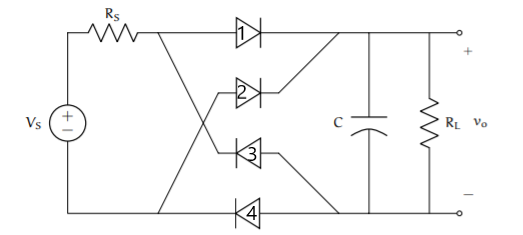
\includegraphics[width=.9\linewidth]{figures/circdiagram.png}
	\caption{Circuit Diagram}
	\label{fig:diagram}
\end{figure}
\section{Materials and Methods}

``This is like a cooking recipe. Include enough detail so that someone can repeat the experiment. It is important that the reader be able to interpret the results knowing the context in which they were obtained.

``The Materials and Methods section should be written in the past tense, since your experiments are completed at the time you are writing your paper.''

Here are some things you don't want to do in this section.

\begin{enumerate}
\item 
Don't simply copy and paste material from my description. 
\item 
Don't simply list the procedure in bullet points (although some lists are fine). I want a description in \emph{your} words.
\item
Don't use a figure from my description unless you properly cite it! A proper citation would be \citep[p.~32]{Picone2018}.
\end{enumerate}

\section{Results}
\label{sec:results}

``To write the results section, use the figures and tables as a guide. Start by outlining, in point form, what you found, going slowly through each part of the figures. Then take the points and group them into paragraphs, and finally order the points within each paragraph. Present the data as fully as possible, including stuff that at the moment does not quite make sense.

``Verbs in the results section are usually in the past tense. Only established scientific knowledge is written about in the present tense, `the world is round,' for example. You cannot presume that your own data are part of the body of established scientific knowledge, and so when you describe your own results, use the past tense, `a band of 1.3 KB was seen,' for example. There are, however, exceptions to this general rule. It is acceptable to say, `Table 3 shows the sizes of the DNA fragments in our preparation.' It is also acceptable to say, `In a 1991 paper, Ebright and coworkers used PCR to mutagenize DNA.' \ldots

``Some readers begin by scanning the figures first. The figures, with the legends, should provide a self-explanatory overview of your data. Decide what the data show, then create figures which highlight the most important points of your paper.

``Tables are used to present repetitive data that is numerical. Graphs or illustrations, collectively called figures, are used to present numerical trends, raw data (like a picture of a gel), or a model that explains your work.

``When you prepare your figures and tables, keep in mind that it is significantly more expensive for journals to publish figures and tables than text, so try to present the data in a way that is worthy of such added expense.''

\begin{table}[bt]
	\begin{tabularx}{1\linewidth}{ lXX }
		\hline
		 & \textbf{RL(Ω)} & \textbf{C (μF)} \\
		\hline
		nominal & $1000$ & $100$ \\
		measured & $993.2$ & $113$ \\
		\hline
	\end{tabularx}
	\caption{Multimeter Measurements}
	\label{tab:Tab1}
\end{table}

\begin{table}[bt]
	\begin{tabularx}{1\linewidth}{ lXXXX }
		\hline
		 & \textbf{Vd1} & \textbf{Vd2} & \textbf{Vd3} & \textbf{Vd4} \\
		\hline
		measured & $0.5$ & $0.6$ & $0.6$ & $0.6$ \\
		\hline
	\end{tabularx}
	\caption{Diode Measurements}
	\label{tab:Tab2}
\end{table}
\section{Discussion}

``This is the section of the paper for you to show off your understanding of the data. You should summarize what you found. Explain how this relates to what others have found. Explain the implications.''

\section{Author Contributions}

You are required to describe each member's contributions to the laboratory exercise and report.

%%% References -------------------------

\bibliographystyle{plainnat}
\bibliography{report}

%%% Appendices -------------------------

\appendix

\section{Appendix: \LaTeX{} Tutorial}\label{sec:latex}

I'm going to teach you how to use \LaTeX{} a little bit. Like how to cite a source, insert a graphic, and build tables. Follow along in the \texttt{report.tex} file.

{\bfseries\color{red} Do not use this appendix as any sort of template for the report! Equations, figures, and tables should appear in the body of the report.} Delete this appendix before submitting your report.

\subsection{Citing a Source}

Let's cite a source. The source must be already saved as a BibTeX file (\texttt{.bib}) in the same directory as the \texttt{.tex} document. I have already created a sample \texttt{report.bib} file. (If you want to add and remove sources to this file, you may use a reference manager like BibDesk on a Mac or JabRef on a PC.)

The next step is to cite the source, inline~\citep{Rowell1997}. And I can easily cite another reference~\citep{Ciesielski1997}.

\subsection{Equations}








\end{document}  